% !Mode:: "TeX:UTF-8" 

\BiChapter{基于贝叶斯网络的克隆变化时一致性维护预测方法}
{Predicting Clone Consistency-Requirement Based on Bayesian Network at Clone Changing Time}

\BiSection{引言}
{Introduction}

由于日益增长的软件开发的需求,开发人员在软件开发过程中经常复用既有代码,从而向系统中引入了大量的克隆代码。克隆代码会随着软件系统演化,在其演化过程中,克隆组内的某一克隆代码片段可能会被软件开发员修改而发生变化。由于克隆组内的克隆片段彼此相似,克隆片段变化可能会导致其所在克隆组未来演化过程中的一致性变化。遗忘这种克隆代码的一致性变化,会引入与之相关的克隆一致性缺陷,从而增大系统的维护代价。本文将由克隆代码变化所导致的其所在克隆组未来演化过程中发生的一致性变化,称为克隆代码变化时的一致性维护需求。在克隆代码变化时时预测克隆代码的一致性维护需求,可以帮助避免克隆代码的一致性缺陷,从而帮助提高软件质量和可维护性。

鉴于此,本章与第三章相似,在定义克隆代码变化时的一致性变化和一致性维护需求的基础上,使用机器学习中的贝叶斯网络方法在克隆代码变化时预测其一致性维护需求。为训练克隆代码变化时一致性预测模型,首先通过构建软件系统的克隆家系来收集系统中所有的克隆变化实例(发生变化的克隆代码)。然后,提取了代码属性、上下文属性和演化属性三组属性值表示克隆代码变化实例。最后,使用贝叶斯网络方法训练机器学习模型,并预测克隆代码变化时的一致性维护需求。在四个开源软件系统上对本章方法进行了评估,实验结果表明本章方法以合理的准确率和召回率有效地预测克隆代码变化时的一致性维护需求。本章所提出的预测方法同样可以帮助开发人员在克隆代码变化时预测克隆代码的一致性,避免克隆变化导致的一致性缺陷,从而提高软件质量和可维护性。

\BiSection{克隆代码变化时一致性维护需求}
{Clone Changing Consistency-Requirement}

\BiSubsection{一致性变化例子}
{An Example of Clone Consistent Change }

在软件开发过程中,复用既有代码是一种常见的软件开发手段,但是也会向软件系统中引入大量的克隆代码。有研究表明软件中的克隆代码可以占到系统代码规模的7\%-23\%\cite{koschke2007survey}。软件中存在的克隆代码不是静止不变的,会随着软件系统进行演化,其演化过程可使用克隆家系进行描述\cite{kim2005empirical}(克隆演化见本文~\ref{ref-evolution}~节)。本文第二章通过分析克隆演化特征发现,在克隆演化过程中,克隆代码的一致性变化往往多于不一致性变化,因此开发人员需要警惕发生变化的克隆代码,并且当发生变化时需要考虑克隆代码的一致性问题。(具体可参考本文~\ref{ref-characteristics}~节)

演化中的克隆变化使得克隆代码变得越来越难以维护,而克隆代码的一致性问题会导致额外的维护代价。当克隆代码发生变化时,程序开发人员需要验证克隆代码的一致性,从而导致维护代价的增加;如果开发人员忘记验证克隆代码的一致性,则可能会向系统中引入新的克隆一致性缺陷在\cite{bettenburg2009empirical} \cite {juergens2009code}。本文第三章研究了克隆代码创建时的一致性维护需求问题,在克隆代码产生时预测克隆代码一致性。在一定程度上可以降低软件的维护代价。但是,值得注意的是,并不是所有的克隆代码都可以被避免。同时,上述方法也无法处理系统中已经存在的克隆代码的一致性变化问题。因此,本章将讨论克隆代码变化时其一致性维护需求问题。

在详细论述本章方法之前,本文先给出一个克隆代码的一致性变化的具体例子,如图~\ref{co-change}~所示。该一致性变化例子来自于软件系统{jEdit}中。在图~\ref{cg1}中给出了$ 3.1.0 $版本中的两个克隆代码片段,它们之间是彼此相似的,可称之为克隆代码。在随着系统演化至$ 3.2.0 $版本时,上述两个克隆代码发生了一致性变化。具体地,$ 3.1.0 $版本中的第9-12行和第15行代码在下一版本$ 3.2.0 $中被开发人员修改。第9-12行,开发人员将{\tt selectionEnd}更改为$ 0 $,并删除了一对花括号。在第15行,开发人员删除了声明语句。如图~\ref{cg2}~所示,这两个被修改的代码片段仍然是彼此相似的克隆代码(仍存在于版本$ 3.2.0 $中的同一克隆组中)。假设程序人员没有对上述两个克隆代码进行一致性维护,这必然会导致克隆代码的一致性缺陷,从而降低软件质量。

\begin{figure}[htbp]
\centering
\subfigure{\label{cg1}}
\addtocounter{subfigure}{-2}
\subfigure[Two clone fragments in one clone group in version $3.1.0$]
{\subfigure[版本$ 3.1.0 $中同一一个克隆组中的两个克隆片段]{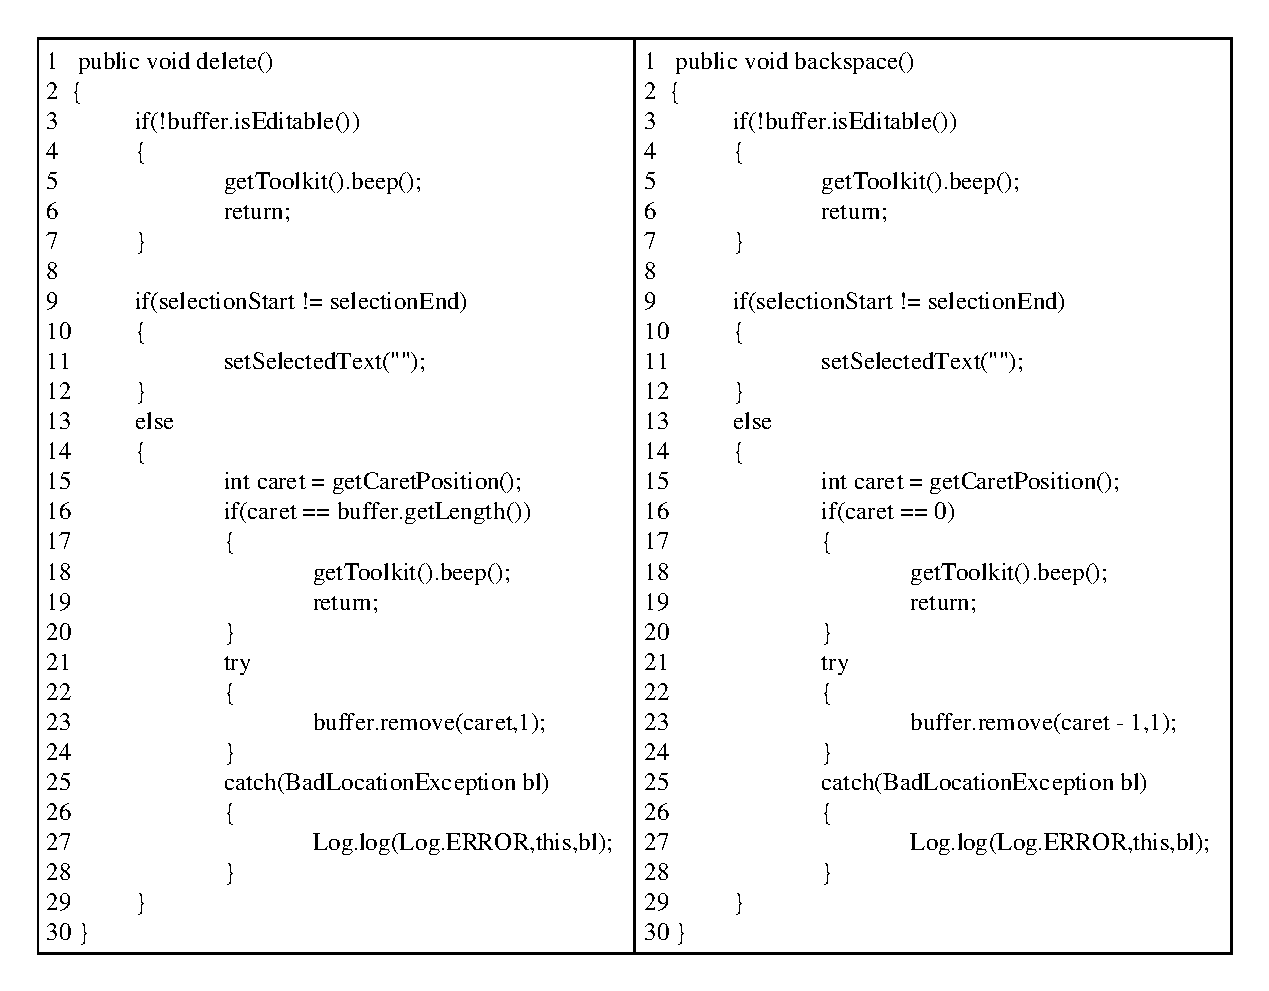
\includegraphics[width=0.8\textwidth]{co-changea.pdf}}}
\subfigure{\label{cg2}}\addtocounter{subfigure}{-2}
\subfigure[Two clone fragments in clone group in version $3.2.0$]
{\subfigure[版本$ 3.2.0 $中克隆组中的两个克隆片段]{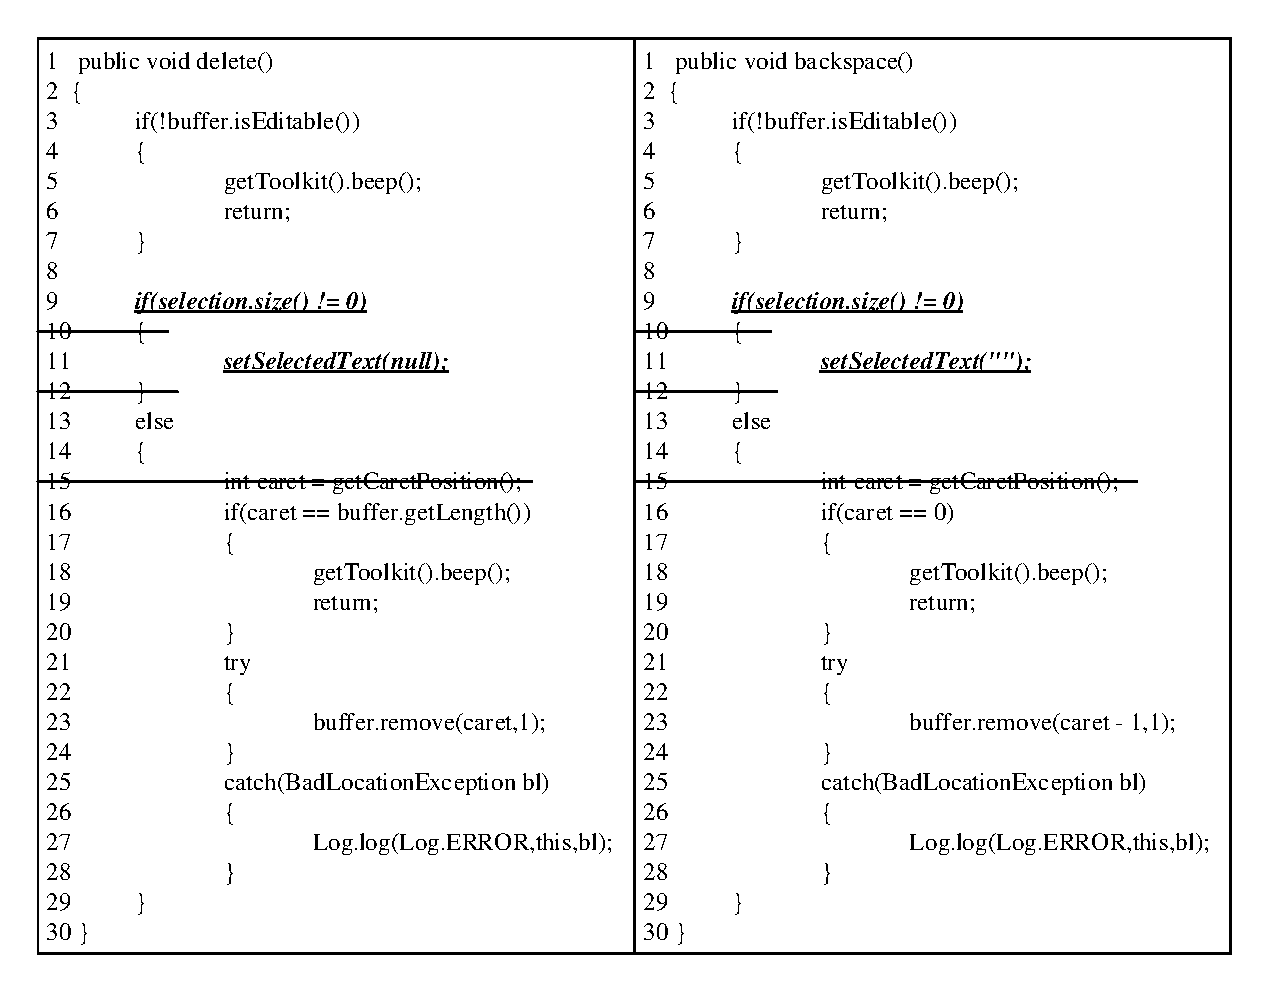
\includegraphics[width=0.8\textwidth]{co-changeb.pdf}}}
\bicaption[co-change]{}{jEdit中的一致性变化的例子}
{Fig.$\!$}{An example of consistent change from jEdit}
\vspace{-1em}
\end{figure}

鉴于此,本章对发生变化的克隆代码进c行一致性预测,在克隆代码变化时,预测克隆代码的一致性维护需求。本章在克隆代码演化的基础上结合克隆代码一致性维护,首先给出了一种克隆代码变化时的一致性变化和一致性维护需求的定义,可以帮助预测克隆变化的一致性维护需求。然后,在第二章研究的基础上重新设计了代码属性、上下文属性和演化属性三组属性表示克隆代码的变化实例。最后,使用贝叶斯网络在克隆代码变化时预测其一致性维护需求。本章方法可以帮助程序开发人员避免克隆一致性缺陷,从而降低克隆代码的一致性维护代价。
%因此,本章方法可可以提高系统的可维护性和软件质量。



%我们通过WEKA \cite{hall2009weka}开发和构建了一个贝叶斯网络作为预测器,并对三个软件项目的预测能力进行了实验。
%我们的实验表明:预测器执行稳定的精确度和召回,对于克隆一致性要求和无一致性的预测,精度范围在70\%到80\%之间,其召回率在63\%和83\%之间。 {\em {我们的实验表明:预测变量的精确度和回忆率对于一致性要求和自由变化实例具有每个存储库的稳定范围;并且为了保持一致性,精度范围在70到80\%之间,其召回率在63和89\%之间。}}此外,每个属性集以其自身的方式对预测能力作出肯定贡献,并且这些属性集中的任何属性集的缺失都可能不利地影响预测器的回忆能力。 {我们的方法可以集成在IDE中以维护克隆更改,这可以避免克隆一致性缺陷。}
%本文的贡献如下:
%\begin {itemize}
%\item 我们提出一种方法来预测克隆组中发生克隆变化所致的一致变化的需要。
%\item 我们基于与克隆系谱相关的信息来识别一组新的属性用于预测。结果表明,这套属性对预测变量的回忆能力有积极影响。
%\item 我们通过对四个开源项目的评估来证明这种预测的可行性。结果表明,我们的方法可以有效预测克隆组的一致变化,具有良好的精度和合理的回忆,并可以帮助提高软件的可靠性通过预测性克隆维护的可重用性。
%\end {itemize}



%在我们的工作中,我们使用克隆检测工具{\em NiCad}来检测来自软件库的克隆。这里,如果两个(或更多个)克隆片段足够相似,则它们形成克隆组。在{\em NiCad}中,这种相似性度量用UPI(代表{\em unique percentage items})表示。UPI根据代码的百分比定义了两个克隆片段之间的{\em 差异}。例如,值为$ 0.3$的UPI表示这两个克隆片段中的30\%不同;换句话说,它们中的70\%具有相同的代码行。
%在这项工作中,{\em  我们设置一个阈值$tau-{CG}$为$0.3$形成克隆组};即,如果UPI $(c_1, c_2)- 0.3$,两个克隆片段$ c_1 $和$ c_2 $被视为属于同一克隆组。}


\BiSubsection{克隆变化时一致性维护需求定义}
{The Definitions for Clone Changing Consistency-Requirement}

在克隆代码的演化过程中,克隆片段可能会被开发人员修改,从而导致克隆代码的一致性变化,这种克隆代码变化可能会导致克隆一致性缺陷。为了描述克隆代码的这种修改,本章给出克隆代码变化时一致性变化定义,如下所示:


\begin{definition}[变化时一致性变化(Changing Consistent Change)]  
\label{def-changingchange}
给定存在两个克隆代码片段 $CF_1$和 $CF_2$,且它们被分别地修改为$CF'_1$和$CF'_2$。  如果对于一个非常小的阈值$\tau$,克隆代码$CF_1$和$CF_2$的变化满足以下条件,称此变化为{克隆变化时的一致性变化(Changing Consistent Change)} , 
  \[
  \begin{array}[t]{crl}
    \mathit{textSim}(CF_i, CF'_i) < 1 & \forall i \in \{1,2\} &(1) \\
    \multicolumn{2}{c}{| ~\mathit{textSim}(CF_1,CF'_1)  ~-~ \mathit{textSim}(CF_2,CF'_2) ~| ~< ~ \tau}  & (2)
  \end{array}
  \]
\end{definition}

%% \ begin {definition} [$ \ tau $ -Conistent change]
%% \ label {defn-1}
%% {\ em
%%假定两个克隆片段$ c_1 $,$ c_2 $分别修改为$ c'_1 $和$ c'_2 $ %%。我们认为$ c_1 $和$ c_2 $之间的修改是$ \ tau $ - {\ em一致的更改\ /}如果对于某个阈值$ \ tau $,
%% \ [
%% \ begin {array} [t] {l}
%% \ mathit {textSim}(c_i,c'_i)<1 ~~~ \ forall i \ in \ {1,2 \} \\
%% | 〜\ mathit {textSim}(c_1,c'_1)〜| 〜 - 〜|〜\ mathit {textSim}(c_2,c'_2)〜| 〜<〜\ tau
%% \ end {array}
%% \]
%%}
%%注意$ \ mathit {textSim} $是根据NiCad中使用的%%度量实现的相似性度量。 \ textcolor {blue} {在NiCad中,这种相似性度量是以UPI(代表{\ em唯一百分比项目})表示的%%。}
%% \ end {definition}
%% 
  
注意$\mathit {textSim}(c,c')= $ 1 - UPI($ c,c'$),UPI是两个代码片段之间不同的代码行数占总代码行的比例,计算方式同第二章中的计算方式相同。第一个约束条件要求 $ CF_1 $和$CF_2 $同时修改;第二个约束条要求$ CF_1 $和$CF_2$发生满足阈值$\tau$条件下一致性的变化,即对代码片段进行了非常相似且一致的变化。本章中$\tau$取值为$0.003$,要求代码片段之间变化完全一致。

变化时一致性变化,不仅要求克隆代码片段被同时修改,还要求一致的变化。原因在于:在克隆代码变化时,目的是避免克隆变化可能导致的未来演化中的一致性变化,及其因此所引发的克隆一致性缺陷。因此, 不仅要求两个克隆代码片段同时变化,还需要发生相似的变化,否则将会引入克隆一致性缺陷。

在克隆演化过程中,克隆片段的变化必然也会导致克隆组的变化,而克隆组的变化可以使用克隆演化模式进行描述,即一致性变化模式。本文给出演化过程中克隆组的一致性变化模式定义,如下所示:

\begin{definition}
[变化时一致性变化模式( Changing Consistent Change Pattern)] 
\label{def-changingpattern}
在软件版本 $j+1$中存在一个克隆组$CG'$ ,假设克隆组内至少存在两个克隆代码片段$CF'_1$ 和 $CF'_2$可以与映射到上一版本$j$的克隆组$CG$中,且 $CG$中与之对应的克隆代码片段的 $(CF_1,CF_2)$被修改为$(CF'_1,CF'_2)$。如果克隆片段之间的变化( $(CF_1,CF_2)$变化至$(CF'_1,CF'_2)$满足克隆片段的“一致性变化(Consistent Change)”,则称克隆组$CG'$具有一致性变化模式(Consistent Change Pattern)。
\end{definition}

%\begin{definition}[{\bf Consistent/Inconsistent Change Pattern}] 
%  \label{}
%  {\em 
%  Given a threshold $\tau$. A clone group $G'$ in software version $j+1$ possesses {\em\bf consistent change pattern} if there exists a pair of clones $c'_1,$ and $c'_2$  in $G'$ which are mappable to a pair of clones $c_1$ and $c_2$ in a clone group $G$ in version $j$ such that modification of code pairs from $(c_1,c_2)$ to $(c'_1,c'_2)$ is a $\tau$-consistent change. Conversely, we say that clone group $G'$ in version $j+1$ possesses {\em\bf inconsistent change pattern}.
%  } 
%\end{definition}

变化时的一致性变化模式,与其它论文中使用的定义不同,其原因在于:本章目的在于预测克隆代码的一致性所导致的克隆一致性缺陷。为了便于读者更容易理解克隆变化时的一致性维护需求,本章现给出克隆变化实例的定义,如下所示:

%Definition~\ref{defn-2} differs from those used in the earlier work such as \cite{Kim2005,Saha2011}, which identify consistent change by asserting that {\em all} clones evolving from previous version of clone group are detected to be similar by clone detection tools.
%More importantly, we label a clone group with consistent change pattern {\em so long as consistent change (as defined above) occurs for a pair of clones.\/} 
%We believe this definition aligns better with the understanding that as long as there exists a pair of clones that needs consistent change, we should inspect the clones in the clone group when any clone has been modified.
%Consequently, the clone genealogy that we build will be different from that of \cite{Kim2005,Saha2011}. 


\begin{definition}[克隆变化实例( Clone Changing Instance)] 
\label{def-changinginstance}
克隆变化实例:
软件版本 $j$中的一个克隆组$CG$是克隆变化实例,如果克隆组$CG$发生了变化且版本$j+1$ 中至少存在一个克隆组$CG'$与之对应(在同一克隆家系$CGE$中)。 
\end{definition}

%\begin{definition}[{\bf Change Instance}] 
%\label{}
%{\em 
%A clone group $G$ in version $j$ is a {\bf change instance} if at least one clone group $G'$ in version $j+1$ which is connected to $G$ in the clone genealogy possess consistent or inconsistent change pattern. 
%}
%\end{definition}


给定一个克隆变化实例,在其未来的演化过程中,可能会导致克隆组的一致性变化模式。克隆组的一致性变化可能会导致一致性缺陷,从而降低软件质量。因此,在克隆代码变化时,预测其未来演化过程中是否会发生一致性变化,可以避免由克隆变化实例导致的一致性缺陷。本文将克隆变化所导致的一致性变化,称为克隆一致性维护需求。克隆变化时的一致性维护需求定义如下:
%接下来,虽然一致和不一致的更改模式指定克隆如何从一个版本发展到下一个版本,但我们实际上更有兴趣了解一对克隆{\em 是否会在未来}中发生一致的更改。这是因为在实践中,开发人员可能选择延迟做出一致的更改,或者有时他们可能甚至不知道需要进行一致的更改,直到未来出现问题.

\begin{definition}[变化时一致性维护需求(Changing Consistency-Requirement)] 
 \label{def-changingconsistency}
给定版本 $j$中一个克隆变化实例,$CG$满足克隆一致性维护需求(Consistency-Requirement),如果在版本$k$中存在一个克隆实例 $CG'$($k>j$)满足以下条件: (1) 在$CG'$中至少存在两个克隆片段在其克隆家系$CGE$中可以映射到克隆实例 $CG$中, (2) $CG'$ 具有“一致性变化模式”(Consistent Change Pattern)。反之,假如克隆变化实例$CG$ 不满足克隆一致性维护需求条件,称该克隆实例不需要一致性维护(consistency-requirement free,或者consistency-free)。
\end{definition}

%\begin{definition}[{\bf Consistency-Requirement (Free)}] 
%  \label{}
%  {\em 
%A change instance $G$ in software version $j$ satisfies 
%{\bf  consistency-requirement\/} condition if there is a clone group $G'$ in software version $k$, with $k>j$, such that (1) there is at least a pair of clones in $G'$ that is mappable in clone genealogy to a pair of clones in $G$, and (2) $G'$ possesses ``consistent change pattern''. 
%When $G$ does not satisfy consistency-requirement, we say that it is {\bf  consistency-requirement free\/}, or simply {\em consistency-free\/} for short. }
%\end{definition}

最终,可以将本章的的研究问题表述如下:给定一个克隆变化实例,即克隆组中$CG$的克隆代码片段$CF$被修改,确定$CG $是否满足克隆变化时一致性维护需求。

更进一步,根据上述定义克隆变化实例只有两种状态:满足和不满足一致性维护需求。我们将变化实例的一致性要求的预测转化为分类问题。本章克隆变化时的克隆一致性需求预测问题可转换为一个典型的分类问题,因此使用机器学习模型解决此分类问题,具体方法见下文。



\BiSection{克隆变化时一致性维护需求预测框架} 
{The Framework of Clone Changing Consistency-Requirement}
我们的方法可以分为两个步骤:构建步骤和预测步骤。在构建步骤中,我们首先从软件存储库收集所有{\em 更改实例}以构建和训练贝叶斯网络。在预测步骤中,开发人员可以使用我们构造的贝叶斯网络来预测一致性要求。我们的预测过程的框架如图~\ref{framework4}~所示。

\begin{figure}[htbp]
\centering
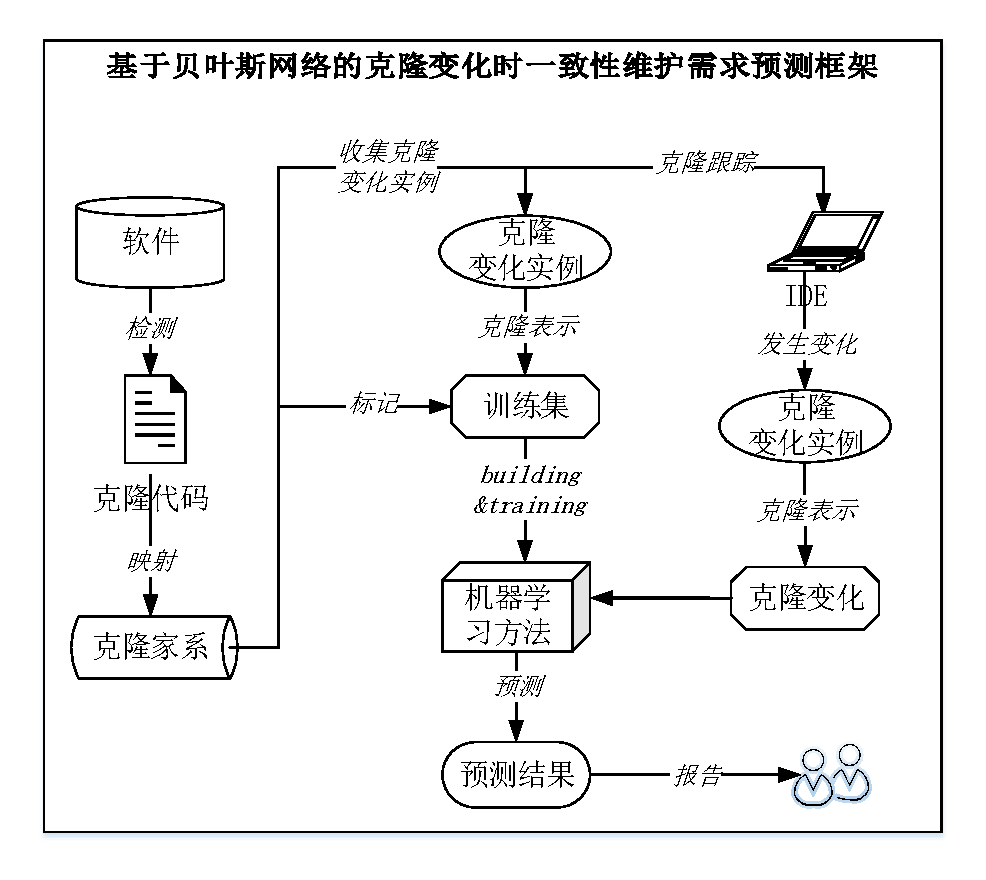
\includegraphics[width = 0.8\textwidth]{framework4.pdf}
\bicaption[framework4]{}{一个克隆系谱的例子}
{Fig.$\!$}{The framework for clone changing consistency-requirement prediction based on Bayesian network}
\vspace{-1em}
\end{figure}

在构建步骤中,我们从考虑的主题软件的存储库收集所有一致和不一致的更改实例,并构建和训练贝叶斯网络模型以预测克隆一致性要求和无一致性。具体来说,我们使用NiCad来检测软件版本中的所有克隆,并通过在相邻版本的克隆组之间进行映射来构建克隆系谱。之后,我们为每个克隆组提取三组属性,用于训练和测试模型。在构建预测模型时,我们采用WEKA包提供的贝叶斯网络实现。接下来,在预测步骤中,开发人员可以使用我们的模型进行预测{({\ sffamily这只是一致性需求预测,关于无一致性预测如何?}}

克隆组是否需要(或不需要)一致的更改;具体地,在该组中是否存在至少两个克隆一致地发展到未来。如果模型预测克隆组需要一致的更改,开发人员将从系统收到关于需要持续保持克隆的警报;类似地,如果模型预测不需要一致性改变,则开发者将同样地被警告,使得他们可以更自信地自由地进行他们的改变。{克隆组是否需要一致的更改,其中一些克隆已更改,对于未来组中的至少两个克隆。如果克隆组将遇到一致的更改,我们可以警告开发人员一致的维护;如果没有,开发人员可以更自由地进行更改。}

通常,软件缺陷的预测需要知道某些代码属性,其被编码为贝叶斯网络(可观察事件)的节点。
在复制和粘贴克隆片段时,使用一些代码属性(将在后面描述)来预测克隆一致性要求(Wang2012,Wang2014)。我们在这项工作中也这样做。除了使用他们确定的一些属性,特别是在使用他们的第一组属性,我们还考虑克隆系谱的进化属性,因为我们相信历史进化信息为我们的预测提供线索。

具体来说,在构建贝叶斯网络模型时,我们从克隆组中提取三组属性:代码属性,上下文属性和进化属性。同时,还将记录关于特定克隆变化的信息。通过它们,贝叶斯网络将被训练以给出克隆改变相对于其克隆组的一致性要求(和免费)的概率。

\BiSection {克隆变化实例收集与表示}
{Collection and Representation for Clone Change Instances}

\BiSubsection {\bf 收集克隆更改实例}
{Collecting Clone Change Instances} 

我们基于整个软件仓库中提供的信息构建和训练我们的预测模型。具体来说,通过从存储库的整个历史构建克隆系谱,我们能够提取关于在每个版本的软件可用的代码克隆的历史数据。虽然我们遵循在\cite {}{Kim2005}中提供的方法来构建克隆系谱,但是我们不同于他们在我们收集的克隆组模式中的工作,如在~\ref{sec:requirement}~中详细描述的。

(1){\bf 检测代码克隆和构建克隆系谱} 我们使用NiCad检测所有克隆,并形成克隆组,从每个版本的实验软件。接下来,我们{\em 映射}克隆组之间的每对相邻版本构建克隆系谱。具体来说,我们首先为每个克隆片段生成一个{\em clone region descriptor} $ \mathit {CRD} $ - 其细节在\cite {}{Duala2010}中描述。然后我们使用称为{\emph 基于CRD的克隆组映射算法}的映射算法来映射两个连续版本之间的所有克隆片段和克隆组。基于地图结果,我们为软件库建立克隆系谱。这个工作的细节可以在\cite{} {Ci2013}中找到。

(2){\bf 收集更改实例和标识克隆模式}.对于每个克隆组,我们确定其克隆模式。这需要检查该克隆组与其直接前趋者(如由克隆系谱提供的)之间的一致变化。一致变化的实际计算在定义~\ref {defn-1}~中指定。接下来,克隆组将被它拥有的改变模式标记(如定义~\ ref{defn-2}~中所指定)。

最后,我们从模式标记的克隆组中识别{\em 更改实例}。此外,对于每个变化实例,我们提取与在该实例上已经进行的修改的种类有关的信息。

\BiSubsection {\bf 特征提取}
{Extracting Change Instance Attributes} 

在模型训练中,每个变化实例由它们表示属性。我们从每个克隆实例中选择了三组属性作为贝叶斯网络模型的输入。这三组捕获克隆组的三个不同方面。它们是代码属性,上下文属性和进化属性。
前两组与Wang等人提供的类似。 \cite{} {Wang2014},而最后一个属性集是新添加的,旨在捕获克隆进化属性。

(1){Code attributes}
这些属性捕获组中代码克隆的特征。属性类似于\cite{} {Wang2012}中收集的属性。主要区别在于它们的计算:Wang et al。 从两个代码聚集的属性:复制和粘贴代码。这里,我们计算每个属性的平均值,当需要时。因此,我们的属性包括代码行的平均数,参数的平均数,调用调用的平均数。此外,我们有:

\begin{itemize}
\item Clone Group Size: 
The number of code fragments in the clone group.
%% \item Average Code Lines: The average number of code lines for all
%%  clone fragments in clone group.
\item Average Number of Halstead: 
The average number of Halstead for all clone fragments in clone group. The Halstead includes the number of distinct operators, number of distinct operands, total number of operators, total number of operands.
%% \item Average Number of Parameters: The average number of parameters
%%   for all clone fragments in the clone group.
\item Average Number of Important Syntactic Constructs: 
For each important syntactic construct (such as \verb+if+, \verb+while+, etc.), we compute the average number of occurrences of the construct for all clone fragments of clone group.
%% \item Average Number of Invocations: The average number of method
%%   invocations for all clone fragments in the clone group, which
%%   includes all invocations, library invocations, local invocations,
%%   and other invocations.
\end{itemize}

(2)Context attributes

该集合包含克隆组中克隆的上下文信息,其中一些类似于Wang等人收集的那些。 在\cite{} {Wang2012}中,主要的区别在于我们计算克隆组中的值,而不仅仅是两个克隆。此外,我们添加了几个属性来描述克隆上下文,例如克隆相似性,参数类型和块信息等。这里是属性列表:

\begin{itemize}

\item Average Clone Similarity: 
The average similarity value between each pair of clones in the clone group. 

\item Locality of Clones: 
This flag determines if all the clone fragments reside in the same file. 

\item Average File Name Similarity : 
There are two attributes to average file name similarity: the real similarity and the masked similarity. 
The mask similarity is a flag indicating if all clones exist in one file. 
In the case when not all the clones are in one file, the real similarity is the average of the similarity measure between the names of the files containing clones. 
Here, Levenshtein distance-based similarity \cite{Navarro2001} is used. 
  
\item Average Method Name Similarity: 
This is the average of the similarity between the names of the methods in which a clone in the clone group belongs.

\item Average Sum of Parameter Similarity (ASPS): 
First, we compute the ``sum of parameter similarity'' (SPS) for each clone pair in the group, as follows: Let $M_1$ and $M_2$ be the two clones with parameters ($P_1$, $P_2$, $\ldots$, $P_m$) and ($Q_1$, $Q_2$, $\ldots$, $Q_n$) respectively. 
We define SPS to be: $\sum_{i=1}^{m}\sum_{j=1}^{n} \mathit{Sim}(P_i,Q_j)$. 
The final ASPS is the average of SPS's.

\item Average Sum of Parameter Type Similarity (ASPTS): 
Similar to ASPS measurement, but applying to parameter type names.

\item Average Maximal of Parameter Similarity (AMPS): 
For each pair of clones $pc$, we compute the {\em maximal of parameter similarity (MPS)}, which is defined as: $\mathit{Max}(\mathit{Sim}(P_i,Q_j))$, where $1\leq i\leq m$, $1\leq j\leq n$, and $\mathit{Sim}(x, y)$ denotes the similarity between string $x$ and string $y$. 
The final AMPS is the average of these MPS's. 

\item ``Is-same-block'' Flag:  
This flag indicates if all the clones are enclosed within block statements of the same syntax.
\end{itemize}

(3)Evolution attributes

最后一组包含关于家谱的属性。克隆组的特征,并且它涉及克隆组如何演变为当前版本。在整个进化历史中,对于一些修订可以存在变化实例,并且还可以经历多于一个变化。这些可以从克隆系谱中提取。 属性是:
  %对于这些指标,我们使用克隆生命周期,其生命周期中的克隆模式数量作为指标:
  %

\begin{itemize}
\item Clone Group Age: 
The number of versions the clone group has existed in this repository until now.

\item Number of Clone Patterns: 
The number of clone patterns which this clone group experiences until now since its inception. 
For each clone pattern, we determine the number of occurrences of this pattern in the clone group's history.

\item Current Pattern: 
The clone pattern of this clone group, as derived from its change (or unchanged) from the previous version (as formally specified in Definition~\ref{defn-2}.)

\item Summaries of Clone Changes: 
The number of changes of this clone group since its inception until the current version.
For each important code syntax (as specified in the set of code attributes), we capture two pieces of information: We summarize the number of times in the clone genealogy (till the present version) that the syntax experiences an increase (and decrease) in its value from one version to the next immediate version. 
For instance, suppose that from the clone genealogy, we discover that a clone group originates in version $i$, and evolves till current version $j$ (where $j > i$). 
We then compare the {\em changes} in the average number of \verb+if+ statements (one of the clone attributes) between two successive versions: versions $i$ and $i+1$, $\cdots$, versions  $j-1$ and $j$. 
This returns to us a series containing positive and negative numbers.
We then record the total number of positives and negatives, forming two summaries associated with \verb+if+statements.
\end{itemize}

\noindent
{\bf Change information.} 
对于每个更改实例,我们还收集有关更改实例中对克隆进行的更改的信息,当它从当前版本发展到下一个版本时。

\begin{itemize}
\item Current Clone Change: 
The change of this clone group from the current version to the immediate next.  
We capture this change for each important syntactic construct.
\end{itemize}

\BiSection {训练与预测}
{Training and Predicting} 

\BiSubsection {训练}
{Training} 
对于每个主题知识库,我们通过收集其变化实例的属性来构建训练数据集。所需的最后一个准备工作是与每个实例关联其一致性 - 要求/无一致性指示,如定义~\ref{defn-4}~中定义。 其中一些将用于训练模型,其他将被用作预测验证的基础真理。最后,形成的数据集将提供给WEKA以开发用于预测的贝叶斯网络模型。在训练模型中,贝叶斯网络的节点表示属性,边缘是属性之间的条件依赖性。



我们应用贝叶斯网络学习技术来解决它。
贝叶斯网络是表示一组随机事件及其条件依赖性的概率图形模型。
形式上,它是一个有向的非循环图,使得其节点表示随机事件,其边缘表示两个节点(事件)之间的条件依赖关系。不连接的两个节点表示有条件地彼此独立的两个事件。
与每个节点相关联的是概率函数,其根据与节点父事件相关联的值计算由节点表示的事件的概率。
有关详细信息,请参阅热门读者\ cite {Pearl1985}



%We apply Bayesian network learning technique to address it. 
%A Bayesian network is a probabilistic graphical model representing a set of random events and their conditional dependencies. 
%Formally, it is a directed acyclic graph such that its nodes represent random events, and its edges represent conditional dependencies between two nodes (events); Two nodes which are not connected represent two events that are conditionally independent of each other.
%Associated with each node is a probability function that computes the probability of the event represented by the node from the values associated with the nodes parent events. 
%We refer avid readers to \cite{Pearl1985} for details.

\BiSubsection {预测}
{Predicting} 
在此步骤中,当现有克隆组发生更改时,软件维护人员可以使用我们的预测变量来预测克隆一致性。如图~\ref{}~所示,我们的方法可以集成到一个IDE,如eclipse,可以保持克隆在开发阶段的变化。运行预测变量需要跟踪克隆在软件进化及其变化中的支持。一旦检测到克隆更改,该工具将提取与此更改实例相关的所有属性,预测其一致性要求,并通知开发人员。
根据预测,开发者因此可以根据需要一致地保持克隆。

这需要IDE提供两个基本功能。第一个功能要求开发人员跟踪克隆及其关联的克隆组,第二个功能需要IDE监控克隆的更改。当开发人员可以跟踪和监视代码克隆时,预测变量可以预测克隆发生变化时一致性要求的可能性。 {\emph {跟踪克隆和监控克隆更改}。首先,我们跟踪克隆及其在IDE中的更改。 \underline {CRD的方法}可以应用于跟踪克隆及其更改。 \emph {提取更改克隆属性和预测一致性要求。}当克隆发生更改时,我们从其关联的克隆组中提取属性。之后,我们将这些数据放入我们的训练模型中,以预测这种一致性要求。 \emph {向开发人员发出警告信号}。我们的预测器将提供描述此更改实例需要一致性要求的概率的分数(介于0和1之间)。这将有助于开发人员考虑是否更改同一组中的克隆。

\BiSection{实验结果和分析}
{EXPERIMENTS}

\BiSubsection{实验设置}
{Methodology}

我们对四个开源的仓库进行了实验项目。表~\ref {}提供了这些项目的详细信息。从表中可以看出,每个项目有数百个更改实例,范围从159到1040个,项目{\em  jEdit}是最小的存储库。其中,满足一致性要求(即,导致克隆组在未来一致的改变)的改变实例的数量显示在列3中,而列2反映了一致性要求自由的改变实例的数量 ,do {\em not }导致任何一致的更改)。
更改满足一致性要求的实例需占用33\%\~\% 5\%到74 \%的所有更改实例。

\begin{table}[htbp]
\bicaption[wdwfas1]{}{符合研究生院绘图规范的表格}{Table$\!$}{The four open source projects for experiment}
\vspace{0.5em}\centering\wuhao
\begin{tabular}{cccc}
\toprule[1.5pt]
~\multirow{3}{*}{\textbf{Project}}& \multicolumn{2}{c}{\textbf{Number (Percentage) of Change Instances}} & \multirow{3}{*}{\textbf{Total}}\\ 
 \cline{2-3}
 ~& \textbf{Consistency-} &\textbf{Meeting} & ~\\
 &\textbf{Requirement Free}&\textbf{Consistency-Requirement}&\\
\midrule[1pt]
ArgoUML&288(67.45\%)&139(32.55\%)&427\\
jEdit&78(49.06\%)&81(50.94\%)&159\\
jFreeChart&452(43.46\%)&588(56.54\%)&1040\\
Tuxguitar&91(25.71\%)&263(74.29\%)&354\\
\bottomrule[1.5pt]
\end{tabular}
\end{table}

%表~\ ref{}~显示从三个项目收集的变更实例的大小的统计信息。中间列显示收集的至少一半的更改实例的大小为2。因此,虽然克隆是丰富的,但它们对系统的引入并不猖獗。{\em  ArgoUML}和{\em jFreeChart}确实有一些超大克隆组; 这些预期在数量上是小的,并且克隆的尺寸也小。

%\begin{table}[htbp]
%\bicaption[table1]{}{符合研究生院绘图规范的表格}{Table$\!$}{Statistics of the size of clone change instances}
%\vspace{0.5em}\centering\wuhao
%\begin{tabular}{ccccc}
%\toprule[1.5pt]
%\textbf{Project}&\textbf{Total}&\textbf{Mean}&\textbf{Standard Deviation}&\textbf{Median}\\ \hline
%\midrule[1pt]
%ArgoUML&427&7.5.9271&	26.22377&2\\ \hline
%jEdit&159&	2.46541&	0.9125&2\\ \hline
%jFreeChart&1040&	7.85288&	26.92378&2\\ \hline
%Tuxguitar&354&	3.40395	&3.45232&2\\ 
%\bottomrule[1.5pt]
%\end{tabular}
%\end{table}

%表~\ref{}描述了更改实例的年龄的统计信息。如前所述,变更实例的年龄是自成立以来所经历的软件版本控制的数量(从$ 0 $计算)。一般来说,更改实例的年龄较小。考虑到变更实例的性质,他们将在当前版本中进行一些代码更改,这个统计数据显示大多数克隆组开始在早期体验代码更改。因此,我们尽可能早地执行一致性要求可满足性的预测变得更相关。

%\begin{table}[htbp]
%\bicaption[dffhg1]{}{符合研究生院绘图规范的表格}{Table$\!$}{Statistics on ages of clone change instances}
%\vspace{0.5em}\centering\wuhao
%\begin{tabular}{ccccc}
%\toprule[1.5pt]
%\textbf{Project}&\textbf{Total}&\textbf{Mean}&\textbf{Standard Deviation}&\textbf{Median}\\ \hline
%\midrule[1pt]
%ArgoUML&427&2.09368&2.33078&1\\ \hline
%jEdit&159&4.48428&3.64371&3\\ \hline	
%jFreeChart&1040&4.93462&4.99543&3\\ \hline	
%Tuxguitar&354&1.5565&1.50294&1\\ \hline	
%\bottomrule[1.5pt]
%\end{tabular}
%\end{table}

我们使用WEKA包建立和培训贝叶斯网络预测模型。WEKA是一个非常灵活和易于使用的数据挖掘工具,包含几种分类/预测方法。在构建我们的模型中,我们选择{\em K2}用于学习网络结构的算法,并且一旦结构已经被学习,使用{\em  SimpleEstimator}来估计贝叶斯网络的条件概率表。贝叶斯网络中的父节点的最大数目被设置为$ 4 $,以便适应属性之间的可能的依赖性,同时不过度消耗模型构造所需的过多的存储器和时间。对于每个克隆更改实例,模型将输出一个值,即其{\em consistency-requirement}的概率。接近$ 1 $的概率值意味着由改变实例经历的当前改变满足{\em consistency-requirement}准则的可能性很高。另一方面,更接近$ 0 $的值意味着这个变化实例很可能是{\em consistency-requirement free}。

基于推断的概率,我们的实验可以自然分为两部分:满足一致性要求和满足无一致性。对于满足一致性要求的更改实例,我们使用{\em Waring Rate,Precision和Recall}来评估我们的方法,该方法尝试警告开发人员可能有一致的更改。另一方面,我们使用{\em Recommendation Rate,Precision and Recall},当克隆变化被推断为无一致性时,尝试推荐开发人员自由地进行任何改变,具有高概率。这些标准的定义在接下来的两个小节中描述。

类似于\cite{} {Wang2012}中的工作,我们从三个不同的角度评估我们的预测的质量。首先,{\em 有效性实验}:我们利用从三个项目中的每一个提取的所有属性来训练和测试模型,并评估预测的质量。第二,{\em 属性集实验}:我们评估三个贡献属性集中的每一个对预测质量的影响。最后,{\em 跨项目实验}:当使用从其他项目提取的数据构建预测模型时,我们评估项目的预测质量。

%我们在具有Intel(R)Core(TM)i5-4210M CPU @ 2.60GHz和8G RAM的桌面上运行我们的实验。每个实验花费不到一分钟的模型构建,交叉验证少于5分钟。大多数实验时间花费在数据准备,包括家谱建构和克隆变化实例收集,其范围在5至30分钟之间。然而,我们注意到,在实践中,克隆系谱构建和变更实例收集将逐步执行,随着软件发展到新版本。因此,数据准备的开销将不是实际问题。

\BiSubsection{一致性实验}
{Consistency-Requirement Experiment}

在本实验中,我们计算以下三个指标来评估我们的模型的一致性要求的可预测性:
\begin{itemize}
\item \textbf{Warning Rate (WR)}: 
This percentage indicates the number of change instances that our model predicts to have met consistency-requirement, and thus warns developers to check for possible consistent change.
It is computed as the ratio of the number of warning raised by the model to all change instances tested. 

\item \textbf{Precision}: 
This assesses the accuracy of the model when it predicts that a change instance under test meets the consistency requirement. 
It is computed as the ratio of the number of {\em correct} predictions of change instances meeting consistency-requirement to the number of predictions made by the model about change instances meeting consistency-requirement.

\item \textbf{Recall}: 
This assesses the effectiveness of the model in discovering all change instances meeting consistency-requirement.
It is computed as the ratio of the number of {\em correct} predictions of change instances meeting consistency-requirement to total number of change instances meeting consistency-requirement (i.e., ground truth).
\end{itemize}

\BiSubsubsection{全属性组实验}
{Effectiveness Experiment}

在这个实验中,我们为四个项目中的每一个构建不同的模型。每当模型预测变化实例满足一致性要求时,它也提供关于该预测的有效性的概率。 因此,我们可以对该概率值设置阈值,使得我们接受该预测是有效的(仅当相关联的概率值至少等于阈值时)。在这种情况下,模型将认为测试中的变更实例满足一致性要求,并向开发人员发出警告。

因此,我们将阈值设置为不同的值来研究它对预测有效性的影响。阈值设置从0.9到0.5,表~\ref{}描述了我们对三个软件的预测的有效性存储库。表中的每一行指示在特定阈值下的预测的质量。此外,我们使用交叉验证$ 10 $ -folds来训练和测试我们的预测变量。

\begin{table}[htbp]
\bicaption[table1]{}{符合研究生院绘图规范的表格}{Table$\!$}{EFFECTIVENESS OF PREDICTORS ON Four OPEN SOURCE PROJECTS}
\vspace{0.5em}\centering\wuhao
\begin{tabular}{ccccc}
\toprule[1.5pt]
\textbf{Project}&\textbf{Threshold}&\textbf{WR(\%)}&\textbf{Precision(\%)}&\textbf{Recall(\%)}\\

\midrule[1pt]
 \multirow{5}{*}{ArgoUML}
&0.9&	20.14&	69.77&	43.17\\
&0.8&	21.31&	68.13&	44.60\\
&0.7&	24.12&	65.05&	48.20\\
&0.6&	24.59&	63.81&	48.20\\
&0.5&	25.29&	62.04&	48.20\\
\hline
\multirow{5}{*}{jEdit}
&0.9&	43.40&	73.91&	62.96\\
&0.8&	47.17&	70.67&	65.43\\
&0.7&	49.06&	70.51&	67.90\\
&0.6&	50.31&	70.00&	69.14\\
&0.5&	50.94&	69.14&	69.14\\
\hline
\multirow{5}{*}{jFreeChart}
&0.9&	52.50&	82.05&	76.19\\
&0.8&	55.19&	81.36&	79.42\\
&0.7&	56.83&	80.71&	81.12\\
&0.6&	58.65&	80.33&	83.33\\
&0.5&	60.10&	79.68&	84.69\\
\hline
\multirow{5}{*}{Tuxguitar}
&0.9	&76.55&   80.44&	82.89\\
&0.8	&78.53&	80.22&	84.79\\
&0.7	&80.51&	80.00&	86.69\\
&0.6	&81.64&	79.24&	87.07\\
&0.5    &83.33&	79.32&	88.97\\
\bottomrule[1.5pt]
\end{tabular}
\end{table}

创建的模型在预测项目{\em jFreeChart}和{\em Tuxguitar}的一致性要求满足方面非常有效,其中预测的精确度和回忆在80\%左右悬停。它执行相当不错,虽然不是那么好,对于{\em jEdit}资源库。这可能是因为存储库的规模较小,但需要进一步调查。尽管{\em  ArgoUML}没有像其他存储库一样的良好预测,但它仍然可以预测精度在65\%左右的需求,并回忆在45\%左右。对于所有的项目,我们的模型产生了相当合理的警告率;它围绕满足一致性要求的变更实例的百分比(如表~\ ref {}~中所列)。

虽然阈值的变化确实影响精度和召回,它对召回的影响比对精度。这意味着,创建的模型在提供中相当稳定,但可以进一步改进其回忆能力。这意味着开发人员可以非常自信地依赖于预测变量的警告,但可能需要其他方法来帮助进一步识别预测变量保持沉默的情况。一个简单的改进是建立模型以预测和警告一致性无需要求的更改实例,从而减少更改实例的数量,没有任何警告(如Wang等人在\cite{}{Wang2014}中所做的)。然而,仍需进一步调查以提高召回率。

\BiSubsubsection{属性组实验}
{Attribute Set Experiment}

本实验是为了确定三者的影响而进行的属性集对训练模型的预测能力。我们对相同的软件存储库进行了实验,但{\em 排除了每个实验的三个属性集合。}表~\ ref{}~显示分别剥离代码属性,上下文属性和进化属性的结果。然后将这些结果中的每一个与具有存在的所有属性(列3至5)获得的结果进行比较。

正如上面的文章,我们使用{三组属性}来预测一致性 - 退休。 为了研究属性组的贡献,我们分别删除每个组(除了当前的变化),其命名为:{\em without code,without context,without evolution}。 我们不会删除当前的更改,因为我们将使用此更改来预测每个实验的一致性要求。 对于每个实验,我们固定阈值从0.9到0.5,并查看精度和回忆如何变化。 我们还使用WEKA来评估我们的预测与10折交叉验证。

\begin{table}[htbp]
\bicaption[table1]{}{符合研究生院绘图规范的表格}
{Table$\!$}{The Significance of each attribute set}
\vspace{0.5em}\centering\wuhao
\begin{tabular}{cccccccccccccc}
\toprule[1.5pt]
\multirow{2}{*}{\textbf{Project}}&\multirow{2}{*}{\textbf{Threshold}}&\multicolumn{3}{c}{\textbf{All(\%)}}&\multicolumn{3}{c}{\textbf{Without Code(\%)}}&\multicolumn{3}{c}{\textbf{Without Context(\%)}}&\multicolumn{3}{c}{\textbf{Without Evolution(\%)}}\\
\cline{3-14}
&&\textbf{WR}&\textbf{Precision}&\textbf{Recall}&\textbf{WR}&\textbf{Precision}&\textbf{Recall}&\textbf{WR}&\textbf{Precision}&\textbf{Recall}&\textbf{WR}&\textbf{Precision}&\textbf{Recall}\\
\midrule[1pt]
ArgoUML&0.9&20.14&	69.77&	43.17&14.29&	73.77&	32.37&17.56&	72.00&	38.85&21.78&	69.89&	46.76\\
jEdit&0.9&	43.40&	73.91&	62.96&	38.99&	75.81&	58.02&	40.88&	75.38&	60.49&	44.03&	71.43&	61.73\\
jFreeChart&0.9&	52.50&	82.05&	76.19&	44.42&	84.63&	66.50&	51.06&	81.92&	73.98&	50.19&	81.42&	72.28\\
Tuxguitar&0.9&	76.55&	80.44&	82.89&	68.64&	79.01&	73.00&	75.14&	78.57&	79.47&	71.75&	80.71&	77.95\\
ArgoUML&0.8&	21.31&	68.13&	44.60&	20.37&	70.11&	43.88&	19.91&	69.41&	42.45&	24.12&	66.02&	48.92\\
jEdit&0.8&	47.17&	70.67&	65.43&	43.40&	72.46&	61.73&	46.54&	70.27&	64.20&	47.80&	69.74&	65.43\\
jFreeChart&0.8&	55.19&	81.36&	79.42&	49.42&	82.10&	71.77&	54.13&	80.99&	77.55&	53.56&	80.07&	75.85\\
Tuxguitar&0.8&	78.53&	80.22&	84.79&	74.01&	79.01&	78.71&	78.53&	78.42&	82.89&	74.01&	80.92&	80.61\\
ArgoUML&0.7&	24.12&	65.05&	48.20&	23.89&	65.69&	48.20&	21.78&	64.52&	43.17&	26.00&	63.96&	51.08\\
jEdit&0.7&	49.06&	70.51&	67.90&	47.17&	70.67&	65.43&	47.80&	71.05&	66.67&	49.69&	68.35&	66.67\\
jFreeChart&0.7&	56.83&	80.71&	81.12&	53.17&	80.83&	76.02&	56.92&	79.39&	79.93&	56.06&	78.39&	77.72\\
Tuxguitar&0.7&	80.51&	80.00&	86.69&	78.25&	78.34&	82.51&	80.79&	77.97&	84.79&	76.55&	80.81&	83.27\\
ArgoUML&0.6&	24.59&	63.81&	48.20&	25.76&	63.64&	50.36&	24.12&	63.11&	46.76&	28.10&	60.00&	51.80\\
jEdit&0.6&	50.31&	70.00&	69.14&	48.43&	71.43&	67.90&	47.80&	71.05&	66.67&	51.57&	65.85&	66.67\\
jFreeChart&0.6&	58.65&	80.33&	83.33&	55.10&	80.10&	78.06&	59.33&	78.12&	81.97&	57.50&	77.93&	79.25\\
Tuxguitar&0.6&	81.64&	79.24&	87.07&	79.94&	78.09&	84.03&	82.20&	77.32&	85.55&	78.53&	80.94&	85.55\\
ArgoUML&0.5&	25.29&	62.04&	48.20&	29.27&	61.60&	55.40&	26.00&	59.46&	47.48&	29.51&	60.32&	54.68\\
jEdit&0.5&	50.94&	69.14&	69.14&	53.46&	69.41&	72.84&	50.94&	67.90&	67.90&	52.83&	65.48&	67.90\\
jFreeChart&0.5&	60.10&	79.68&	84.69&	57.79&	78.20&	79.93&	60.48&	78.06&	83.50&	59.13&	77.56&	81.12\\
Tuxguitar&0.5&	83.33&	79.32&	88.97&	83.33&	77.63&	87.07&	84.18&	76.85&	87.07&	79.66&	80.50&      86.31\\
\bottomrule[1.5pt]
\end{tabular}
\end{table}

为了定量评估每个属性的影响,我们对两个相关对的平均值之间的差异的显着性进行单尾t检验,将零假设设置为全属性样本的精度/回忆的平均值与没有一个样本的样本的平均值相同属性集}。
详情见附录。 t尾结果表明,当代码属性或上下文属性不存在时,一致性要求的回忆能力显着降低。然而,不存在进化的情况的差异不如期望的那么显着。进一步的调查表明,进化属性在{\em ArgoUML}资源库中的召回能力没有显着的帮助。然而,这些属性确实对其他存储库有贡献。需要进一步调查以发现这种差异背后的真实推理。{我们还对没有{\em  ArgoUML}的三个项目(在我们的会议论文中)执行了一个单尾t检验。所有四个项目的t检验结果都不如三个项目。原因是它受到{\em ArgoUML}的严重影响。}然而,很清楚,没有任何一个属性集{\em 不会对训练的模型的精度有任何显着影响}。然而,他们对所训练的模型的召回值都有{\em 具有显着的不利影响}。 \\

此外,我们采用属性选择函数来获得可以用于执行预测的属性的最佳子集。获得的子集根据不同的实验数据(即,不同的软件库)而变化。然后,我们将这些结果与通过使用完整属性集获得的结果进行比较。结果一致地显示所有属性可以比子集属性更好地预测。虽然一些属性可能对实验结果没有显着贡献,但也没有一个具有不利影响。然而,保留这些属性很重要,因为它们的贡献对其他存储库可能变得重要。

\BiSubsubsection{交叉验证实验}
{Cross-Projects Experiment}

为了确保我们的方法可以用于新项目,或者没有足够一致/不一致的更改实例的项目。 使用这样少的数据,我们不能建立有效的预测器。 因此,在最后一个实验中,我们确定使用来自其他软件仓库的数据训练的模型是否可用于预测不同软件存储库的一致性要求满足度。因此,在三个主题仓库中,在本实验中,我们轮流使用来自两个仓库的数据来训练预测模型,并在第三仓库中使用该模型进行预测。表~\ ref {}~描述了实验结果。

\begin{table}[htbp]
\bicaption[table1]{}{符合研究生院绘图规范的表格}{Table$\!$}{Table in agreement of the standard from graduate school}
\vspace{0.5em}\centering\wuhao
\begin{tabular}{ccccc}
\toprule[1.5pt]
{\textbf{Project}}&{\textbf{Threshold}}&{\textbf{WR(\%)}}&{\textbf{Precision(\%)}}&{\textbf{Recall(\%)}}\\

\midrule[1pt]
\multirow{5}{*}{ArgoUML}
&0.9&	40.28&	33.72&	41.73\\
&0.8&	49.88&	35.21&	53.96\\
&0.7&	57.85&	34.01&	60.43\\
&0.6&	62.06&	34.34&	65.47\\
&0.5&	65.34&	34.41&	69.06\\
\hline
\multirow{5}{*}{jEdit}
&0.9&	26.42&	59.52&	30.86\\
&0.8&	31.45&	54.00&	33.33\\
&0.7&	37.11&	54.24&	39.51\\
&0.6&	42.14&	56.72&	46.91\\
&0.5&	45.91&	56.16&	50.62\\
\hline
\multirow{5}{*}{jFreeChart}
&0.9&	21.15&	62.73&	23.47\\
&0.8&	26.44&	62.55&	29.25\\
&0.7&	31.44&	60.86&	33.84\\
&0.6&	35.38&	60.60&	37.93\\
&0.5&	38.65&	59.95&	40.99\\
\hline
\multirow{5}{*}{Tuxguitar}
&0.9&	18.08&	70.31&	17.11\\
&0.8&	22.60&	70.00&	21.29\\
&0.7&	26.27&	70.97&	25.10\\
&0.6&	31.07&	71.82&	30.04\\
&0.5&	35.88&	72.44&	34.98\\
\bottomrule[1.5pt]
\end{tabular}
\end{table}

从表~\ref{}~,我们注意到,当建立和使用预测模型时,所有的精度和召回不同的项目。结合这个结果和第一个实验的结果,我们可以安全地推荐我们的模型在已经发展了相当一段时间的存储库的预测中是有效的,其中存在足够的变化实例。在软件开发的初始阶段,项目可能没有足够的克隆更改实例从其软件库中训练自己的预测。那么我们如何能够对这样一个新的软件开发执行预测呢?

我们的建议如下:在开始软件开发时,我们要求开发人员在创建克隆组时,一直检查一致性要求。跨项目模型可以用于在这一点上谨慎地辅助或由Wang等人建立的模型。 \cite{} {Wang2014}可以在执行复制和粘贴操作时使用。后来,随着软件通过几个版本发展,我们建议通过逐步减少跨项目数据的数量和增加自己的存储库中的数据量来重新训练模型。

\BiSubsection{一致性自由}
{Consistency-Requirement Free Experiment}
在本实验中,我们计算以下三个指标,用于评估我们的模型的一致性无需求的可预测性:
\begin{itemize}
\item \textbf{Recommendation Rate (RR)}: 
This percentage indicates the number of change instances that our model predicts to have met consistency-requirement free, and thus recommends developers to change code clone freely.
It is computed as the ratio of the number of recommendations raised by the model to all change instances tested.
\item \textbf{Precision}: 
This assesses the accuracy of the model when it predicts that a change instance under test to be consistency-free. It is computed as the ratio of the number of {\em correct} predictions of change instances to be consistency-free to the total number of predictions made by the model about change instances to be consistency-free.
\item \textbf{Recall}: 
This assesses the effectiveness of the model in discovering all change instances meeting the requirement of consistency-free.
It is computed as the ratio of the number of {\em correct} predictions of change instances to be consistency-free to total number of change instances meeting the requirement of consistency-free(i.e., ground truth).
\end{itemize}

\BiSubsubsection{全属性组实验}
{Effectiveness Experiment}

在本实验中,模型预测变更实例满足一致性要求空闲,它还提供了关于此预测有效性的概率。由于预测器可以推断克隆变化实例是无一致性的概率,因此我们可以对该报告的概率设置阈值,使得我们接受预测是有效的{仅当相关联的概率值不大于或等于阈值。在这种情况下,模型将给予测试下的变化的置信度满足一致性要求free。开发人员可以自由地更改克隆。在这个实验中,我们监测阈值设置在不同的值,从0.01到0.20,以研究其对预测的有效性的影响。表~\ ref{}~描述了我们对四个软件仓库的预测的有效性。表中的每一行指示在特定阈值下的预测的质量。此外,我们使用交叉验证$ 10 $ -folds来训练和测试我们的预测变量。

\begin{table}[htbp]
\bicaption[table1]{}{符合研究生院绘图规范的表格}
{Table$\!$}{EFFECTIVENESS OF PREDICTORS ON FOUR OPEN SOURCE PROJECTS}
\vspace{0.5em}
\centering
\wuhao
\begin{tabular}{ccccc}
\toprule[1.5pt]
\textbf{Project}&\textbf{Threshold}&\textbf{RR(\%)}&\textbf{Precision(\%)}&\textbf{Recall(\%)}\\
\midrule[1pt]
\multirow{5}{*}{ArgoUML}
&0.01&	51.99&	83.33&	64.24\\
&0.05&	60.42&	82.95&	74.31\\
&0.1&	63.93&	81.32&	77.08\\
&0.15&	65.81&	80.43&	78.47\\
&0.2&	67.45&	80.21&	80.21\\
\hline
\multirow{5}{*}{jEdit}
&0.01&	20.13&	84.38&	34.62\\
&0.05&	30.19&	79.17&	48.72\\
&0.1&	33.96&	74.07&	51.28\\
&0.15&	38.36&	70.49&	55.13\\
&0.2&	39.62&	69.84&	56.41\\
\hline
\multirow{5}{*}{jFreeChart}
&0.01&	28.65&	84.56&	55.75\\
&0.05&	32.50&	83.73&	62.61\\
&0.1&	34.23&	82.02&	64.60\\
&0.15&	35.58&	80.81&	66.15\\
&0.2&	36.06&	80.53&	66.81\\
\hline
\multirow{5}{*}{Tuxguitar}
&0.01&	7.91&	53.57&	16.48\\
&0.05&	9.32&	57.58&	20.88\\
&0.1&	9.89&	54.29&	20.88\\
&0.15&	12.15&	48.84&	23.08\\
&0.2&	13.28&	48.94&	25.27\\
\bottomrule[1.5pt]
\end{tabular}
\end{table}

为项目{\em ArgoUML}和{\em jFreeChart}分别建立的模型对非一致性有非常有效的预测,精度悬停在80\%左右,并回忆到70\%左右。它执行相当不错,虽然不是那么好,对于{\em jEdit}资源库。不幸的是,我们的模型不能预测足够好的{\em Tuxguitar}。这可能是由于更改实例集的小大小(无一致性),但需要进一步调查。对于所有的项目,我们的模型产生了相当合理的建议率。它围绕满足一致性要求的变更实例的百分比(如表~\ref {}中所列)。

虽然阈值的变化确实影响精度和召回,但它对召回的影响比精确度更大。这意味着,创建的模型在提供时相当稳定,但可以进一步改进其回调能力。这意味着开发人员可以相当自信地依靠预测变量发出的警告,但可能需要其他方法来帮助进一步识别预测变量保持沉默的情况。

总之,我们的方法产生的模型提供了一个稳定的预测,合理的精度和召回,给软件开发商带来了对模型产生的推理的回应的信心。一个简单的改进是建立模型以预测和警告一致性无需要求的更改实例,从而减少更改实例的数量,没有任何警告(如Wang等人在\cite{} {Wang2014}中所做的)。然而,仍需进一步调查以提高召回率。

\BiSubsubsection{属性组实验}
{Attribute Set Experiment}
为了评估所选择的三个属性集的影响,我们进行了类似于段落~\ref {}~中所呈现的实验。该实验用于确定三个属性集对训练模型的预测能力的影响。我们对相同的软件存储库进行了实验,但每个实验都排除了三个属性集之一。
表~\ref{}显示了当与所有属性存在({列3})时获得的结果相比,当三个属性集中的一个被省略时({列4到6}),我们的预测的有效性。然后将这些结果中的每一个与所有存在的属性(第3至5列)获得的结果进行比较。

如上文所述,我们使用{三组属性}来预测一致性 - 退出。为了研究属性组的贡献,我们分别删除每个组(除了当前的变化),其命名为:{\em without code,without context,without evolution}。我们不会删除当前的更改,因为我们将使用此更改来预测每个实验的一致性要求。 对于每个实验,我们固定阈值从0.9到0.5,并查看精度和回忆如何变化。我们还使用WEKA来评估我们的预测与10折交叉验证。

\begin{table}[htbp]
\bicaption[sdfj1]{}{符合研究生院绘图规范的表格}{Table$\!$}
{The Significance of each attribute set}
\vspace{0.5em}
\centering
\wuhao
\begin{tabular}{cccccccccccccc}
\toprule[1.5pt]
\multirow{2}{*}{\textbf{Project}}&\multirow{2}{*}{\textbf{Threshold}}&\multicolumn{3}{|c|}{\textbf{All(\%)}}&\multicolumn{3}{|c|}{\textbf{Without Code(\%)}}&\multicolumn{3}{|c|}{\textbf{Without Context(\%)}}&\multicolumn{3}{|c|}{\textbf{Without Evolution(\%)}}\\
\cline{3-14}
&&\textbf{RR}&\textbf{Precision}&\textbf{Recall}&\textbf{RR}&\textbf{Precision}&\textbf{Recall}&\textbf{RR}&\textbf{Precision}&\textbf{Recall}&\textbf{RR}&\textbf{Precision}&\textbf{Recall}\\
\midrule[1pt]
ArgoUML&0.01&	51.99&	83.33&	64.24&	36.77&	89.17&	48.61&	48.01&	83.41&	59.38&	44.03&	85.64&	55.90\\
jEdit&0.01&	20.13&	84.38&	34.62&	18.87&	80.00&	30.77&	22.64&	80.56&	37.18&	23.27&	81.08&	38.46\\
jFreeChart&0.01& 28.65&	84.56&	55.75&	18.94&	89.34&	38.94&	23.75&	84.62&	46.24&	26.73&	84.53&	51.99\\
Tuxguitar&0.01&	7.91&	53.57&	16.48&	3.11&	27.27&	3.30&	5.37&	47.37&	9.89&	9.89&	57.14&	21.98\\
\hline
ArgoUML&0.05&	60.42&	82.95&	74.31&	49.18&	85.71&	62.50&	59.48&	79.92&	70.49&	51.99&	84.23&	64.93\\
jEdit&0.05&	30.19&	79.17&	48.72&	27.04&	79.07&	43.59&	30.19&	77.08&	47.44&	27.04&	79.07&	43.59\\
jFreeChart&0.05&	32.50&	83.73&	62.61&	24.71&	84.44&	48.01&	28.65&	81.54&	53.76&	31.35&	82.21&	59.29\\
Tuxguitar&0.05&	9.32&	57.58&	20.88&	8.19&	41.38&	13.19&	8.19&	48.28&	15.38&	11.58&	51.22&	23.08\\
\hline
ArgoUML&0.1&	63.93&	81.32&	77.08&	56.67&	83.06&	69.79&	63.00&	79.18&	73.96&	58.31&	83.53&	72.22\\
jEdit&0.1&	33.96&	74.07&	51.28&	30.82&	79.59&	50.00&	33.96&	74.07&	51.28&	28.93&	78.26&	46.15\\
jFreeChart&0.1&	34.23&	82.02&	64.60&	28.75&	82.61&	54.65&	31.44&	81.35&	58.85&	32.79&	80.94&	61.06\\
Tuxguitar&0.1&	9.89&	54.29&	20.88&	9.89&	48.57&	18.68&	9.89&	48.57&	18.68&	13.28&	48.94&	25.27\\
\hline
ArgoUML&0.15&	65.81&	80.43&	78.47&	60.42&	83.72&	75.00&	65.11&	78.78&	76.04&	60.66&	83.01&	74.65\\
jEdit&0.15&	38.36&	70.49&	55.13&	33.96&	77.78&	53.85&	36.48&	70.69&	52.56&	32.08&	76.47&	50.00\\
jFreeChart&0.15&	35.58&	80.81&	66.15&	30.77&	81.56&	57.74&	32.88&	81.58&	61.73&	34.62&	78.89&	62.83\\
Tuxguitar&0.15&	12.15&	48.84&	23.08&	11.02&	46.15&	19.78&	10.73&	44.74&	18.68&	14.97&	52.83&	30.77\\
\hline
ArgoUML&0.2&	67.45&	80.21&	80.21&	62.53&	82.77&	76.74&	65.81&	78.65&	76.74&	62.76&	83.21&	77.43\\
jEdit&0.2&	39.62&	69.84&	56.41&	37.11&	76.27&	57.69&	38.36&	70.49&	55.13&	32.70&	76.92&	51.28\\
jFreeChart&0.2&	36.06&	80.53&	66.81&	32.98&	80.17&	60.84&	34.13&	79.72&	62.61&	35.87&	78.02&	64.38\\
Tuxguitar&0.2&	13.28&	48.94&	25.27&	11.86&	45.24&	20.88&	11.86&	42.86&	19.78&	15.82&	55.36&	34.07\\
\bottomrule[1.5pt]
\end{tabular}
\end{table}

为了定量评估每个属性的影响,我们对相关对的两个均值之间的差异执行单尾t检验,将零假设设置为{\em 所有属性样本的精度/回忆的平均值是与没有一组属性的样本相同}。类似于一致性需求预测的情况,我们还进行单尾t检验。细节也在附录部分中显示。根据结果​​,我们有高度的信心,没有一个属性集,其缺席会对他们的精确度产生重大的不利影响。另一方面,缺少这些属性集合中的{\em  any}将对所训练的模型的召回值{\em 具有显着的不利影响}。我们还通过选择从WEKA的属性选择函数获得的属性的最佳子集来建立预测器,旨在探索每个属性的效果。获得的子集会根据不同的实验数据(即不同的软件存储库)而有所不同。
与完整的属性集相比,结果始终表明{\em 全属性预测器具有比子集属性预测器更好的预测能力。}

虽然一些属性可能对实验结果没有显着贡献,但它们都不具有对手影响。因此,我们建议保留构建预测模型中的所有属性,因为一些属性可能会对一些尚未被探索的存储库有重要的贡献。

\BiSubsubsection{交叉验证实验}
{Cross-Projects Experiment}
为了确保我们的方法可以用于新项目,或者没有足够一致/不一致的更改实例的项目。 使用这样少的数据,我们不能建立有效的预测器。 因此,

在这个实验中,我们探讨使用跨项目在预测一致性要求免费的有效性。我们确定使用来自其他软件存储库的数据进行训练的模型是否可用于预测不同软件存储库的一致性要求满足度。四个主题知识库,在这个实验中,具体来说,我们轮流使用来自三个存储库的数据来训练预测模型,并使用模型预测剩余存储库中克隆更改的一致性要求。
表~\ref{changecrossfree}~描述了实验结果。

\begin{table}[htbp]
\bicaption[changecrossfree]{}{项目交叉实验结果}
{Table$\!$}{The Results of Cross-Project Experiment}
\vspace{0.5em}
\centering
\wuhao
\begin{tabular}{ccccc}
\toprule[1.5pt]
{\textbf{Project}}&{\textbf{Threshold}}&{\textbf{RR(\%)}}&{\textbf{Precision(\%)}}&{\textbf{Recall(\%)}}\\
\midrule[1pt]
\multirow{5}{*}{ArgoUML}
&0.01&	6.09&	73.08&	6.60\\
&0.05&	13.11&	76.79&	14.93\\
&0.1&	16.63&	74.65&	18.40\\
&0.15&	20.84&	75.28&	23.26\\
&0.2&	23.19&	71.72&	24.65\\
\hline
\multirow{5}{*}{jEdit}
&0.01&	9.43&	60.00&	11.54\\
&0.05&	21.38&	50.00&	21.79\\
&0.1&	31.45&	44.00&	28.21\\
&0.15&	37.74&	50.00&	38.46\\
&0.2&	42.14&	49.25&	42.31\\
\hline
\multirow{5}{*}{jFreeChart}
&0.01&	26.44&	46.91&	28.54\\
&0.05&	37.60&	46.55&	40.27\\
&0.1&	43.27&	47.56&	47.35\\
&0.15&	46.92&	46.72&	50.44\\
&0.2&	49.33&	46.39&	52.65\\
\hline
\multirow{5}{*}{Tuxguitar}
&0.01&	16.67&	27.12&	17.58\\
&0.05&	33.62&	24.37&	31.87\\
&0.1&	42.37&	26.67&	43.96\\
&0.15&	46.61&	26.67&	48.35\\
&0.2&	49.72&	26.14&	50.55\\
\bottomrule[1.5pt]
\end{tabular}
\end{table}

表~\ref{}表明,与有效实验相比,所有精度和召回都受到影响。结合这个结果和(第一)有效性实验,我们观察到,当从具有足够数量的变化实例的其自己的存储库训练预测模型时,预测模型是有效的;即,当仓库已经演化了相当长的时间。因此,我们建议在软件开发的初期阶段,由于缺乏足够数量的克隆变更实例来良好地训练模型,开发人员可以使用Wang的模型bulit  \cite{} { Wang2014},其检测复制和粘贴操作以避免克隆。在软件进化的几个版本之后,随着来自其自己的存储库的数据量的增加,开发人员可以重新训练模型以预测项目中克隆更改的一致性。

{在软件开发的初始阶段,项目可能没有足够的克隆更改实例从其软件库中训练自己的预测。我们如何才能对这样一个新的软件开发执行预测?} {我们的建议如下:在软件开发的开始,我们要求开发人员在创建克隆组时,一定要检查一致性要求。
跨项目模型可用于在这一点上谨慎地辅助,或由Wang等人建立的模型。 \cite {Wang2014}可以在执行复制和粘贴操作时使用。以后,随着软件通过几个版本的演变,我们建议通过逐步减少跨项目数据量和增加自己的存储库中的数据量来重新训练模型。}

\BiSubsection{讨论}{Discussion}
我们评估了建立的贝叶斯网络模型的预测能力,以预测一致性要求,并为所有克隆更改实例自由。基于我们的实验结果,当他们用所有实例的全属性训练时,我们的模型在一致性要求和无一致性预测上具有有效的预测能力。省略单个属性集的实验揭示了每个属性集在不同程度上对预测模型的质量有显着贡献。因此,应鼓励开发人员沿这三个维度添加其他属性,以进一步提高构建模型的可预测性。

%% \ textcolor {red} {(Why?)}
%% \ textcolor {blue} {通过对一致性要求和免费的属性集评估,结果显示属性集对我们的预测没有不利影响。此外,我们还可以发现,三组属性对于精度和回忆在预测中具有不同但是显着的影响。这使我们建议开发人员可以为自己的目标选择自己的属性。因此,开发人员还应该对每个属性进行更多调查。

跨项目实验表明,预测模型的有效性高度依赖于应用模型的储存库的具体特性。这意味着构建一个“通用”预测模型可能无法预测所有存储库的克隆更改的一致性要求/ - 免费。换句话说,开发人员将需要为不同的存储库创建不同的模型。这当然不是完全可取的,我们认为在这里需要进一步的调查。

来自跨项目存储库的模型的预测能力的无效性还意味着当前方法在模型构建期间在自举中具有限制,因为在软件开发的初期阶段没有足够的改变实例来支持预测模型的构建。在这里,我们建议开发人员在软件开发的早期阶段使用由Wang {\sl et.al.}开发的模型,并且在某些版本中使用我们的模型作为软件。

%\BiSection{相关工作}{Related Work}
%即使由于代码克隆已经被识别为“坏气味”,引起了对它对软件的有害性的讨论。克隆的支持者是有害的,认为它们的存在可以招致额外的维护工作。为此,Lozano和Wermelinger表明,当方法具有clone \cite{} {Lozano2008}时,更改方法的维护工作量可能会显着增加。Barbour et al对在稍后阶段被重新同步的克隆对的未同步改变(称为“后期传播”)表明这种模式与大量的故障相关\cite{}{Barbour2011}。对于克隆有害的对手具有不同的研究结果。例如,Rahman et al。研究开源项目中克隆和缺陷倾向之间的关系,并发现克隆可能比非克隆的代码更少缺陷倾向\cite{}{Rahman2012}。还有其他人对克隆有害性采取中立态度。例如,Kapser和Godfrey描述了几种克隆模式,讨论它们的优点和缺点,并得出结论,存在克隆似乎是合理或甚至有益的设计选项的情况。

%无论代码克隆的存在是否被认为有害,“克隆”作为程序开发活动将持续,因为一般软件开发人员编制代码的方式(出于方便)。对其进化的克隆分析在理解这些克隆中起重要作用。在这方面,Kim et al。提出克隆系谱以描述克隆进化\cite{}{Kim2005}。这形成了克隆进化研究的基础。Kim et al。引入克隆系谱的概念克隆组的进化,并将克隆变化分类为几个“克隆模式”,和两个这样的模式在我们的工作是适应{\em 一致}和{\em 不一致的变化} \cite{} {Kim2005} \cite{} {Saha2011}。
%我们采用克隆系谱的概念,并选择系谱的变异用于预测目的。这将在第4节中详细说明。Saha et al。提出了一种自动为多个版本的克隆提取家谱的方法,并使用一些关键的相似因子识别克隆进化模式。Bakota et al。提出克隆气味的定义,以确定克隆是否与软件缺陷相关\cite{} {Bakota2007}。Krinke发现克隆代码比非克隆代码更稳定,因为平均变化百分比比非克隆\cite{} {Krinke2007}更低。Harder和G o de发现克隆稳定性取决于克隆对应于项目环境\cite{} {Harder2013}的特征。Bettenburg et al。观察到只有1 - 3 \%不一致的更改可以在发布级别引入软件缺陷,并且建议克隆对所研究的软件的发布后质量没有显着影响\cite{}(Bettenburg2009)。还有一些关于克隆一致变化的研究:Krinke的实验揭示,通常代码克隆组的一半更改是不一致的更改\cite{} {Krinke2008}。G o de和Koschke发现大多数克隆很少改变,克隆的无意的不一致的改变的数量很小\cite{} {Gode2011}。

%有一些预测性维护的工作。具体来说,Wang et al。应用贝叶斯网络来预测期望的代码克隆操作是否将触发克隆一致性维护。该预测是从克隆代码结构和克隆操作的上下文中提取的多个属性进行的。相比之下,在我们的工作中,我们采用了克隆操作已经发生的不同应用程序需求,并预测克隆组中的克隆是否需要一致性维护。为此,我们包括与从克隆系谱发现的克隆组特征相关的另外的特征,并且提供克隆一致变化的新定义,其更好地反映一致的变化,即使存在一些不一致的克隆变化。
%其他预测性维护工作包括Hassan,他提出了基于代码变化过程而不是代码的复杂度度量,并发现这些度量是与故障的其他众所周知的历史预测因子相比更好的故障潜在预测因子\cite{}{ Hassan2009}。

%一般来说,克隆维护/管理问题在这个研究社区得到了广泛的应用\cite{}(Roy2014)。克隆维护的一个流行的活动是重构。Krishnan和Tsantalis提出了一种用于统一和重构克隆的方法,其能够发现显着更大数量的可重构克隆\cite{}(Krishnan2014)。Milea et al。基于Deckard \cite{} {Jiang2007},通过向量抽象和具体化技术大规模地发现重构机会\cite{} {Milea014}。同时,已经建立了几个克隆管理工具;例如JSync \cite{} {Nguyen2012},CloneTracker \cite{} {Duala2008},CeDAR \cite{} {Tairas2010}等。历史上,代码克隆的研究可追溯到90年代。在过去的几十年中,一直专注于克隆检测。已经开发了大量的方法和工具,诸如NiCad \cite{} {Roy2008},CCFinder \cite{} {Kamiya2002},iClone \cite{} {Gode2009}等,其通常可以根据所部署的技术被分类成基于文本,基于令牌,抽象语法树,基于程序依赖图,基于度量等。基于Text的NiCad是我们克隆检测工作中使用的工具;它可以产生高精度的克隆和召回\cite{} {Roy2008}。其他流行的工具包括:CCFinder用于有效检测基于令牌的克隆,以及用于识别软件的特定特征\cite{}{Kamiya2002}。
%iClone是基于后缀树的增量克隆检测技术,其比非增量方法需要相当少的时间。
%有兴趣的读者可以参考\cite{} {Rattan2013},基于一整套213篇文章详细检查克隆检测。

%\BiSection{威胁}{Related Work}
%作为一个实证研究,我们的实验结果受到两个有效威胁。首先,构建有效性的威胁关注在我们的实验的构建和评估中使用的度量是否适当。这里有两个潜在的威胁:(1)我们对克隆组的“一致改变”模式的定义可能不是最准确,因为克隆组可以具有多于两个克隆,在克隆组中留下一些克隆不真正匹配模式条件。然而,这不是真正意义重大,有两个原因:在存储库中发现的大多数克隆组的大小为2;此外,我们认为,当需要进行一致性检查时,开发人员应该检查组中的所有克隆是否一致。(2)我们通过所有克隆从一个版本到下一个版本的平均变化近似实际代码变化。这可能不能很好地反映实际的代码更改。我们对这个论点的辩护是,一致性检查仅在软件即将升级到新版本之前进行,而不是每当组中的一段代码改性。因此,预测只有在几乎所有修改时才开始到克隆,并且使用变化的平均值是最适当的度量。

%第二,关于我们的结果可能不会这样.推广到更广泛的软件存储库,我们注意到我们在构建模型中采用了一个整体视图:我们不仅考虑了代码属性,克隆上下文,还包括克隆组的历史,在构建模型的输入。这意味着构建的预测模型是针对个体存储库定制的,因此在概念上是一般的。

%NiCad作为我们的克隆检测工具,可以从软件源代码中产品克隆组。克隆组的大小对于不同的项目是非常不同的。大多数克隆组只有两个克隆片段,也有一些是相当大的。对于更大的克隆组,我们的预测模型可能不能很好地处理。在将来,我们将考虑不同大小的克隆组使用不同的属性。并且,还要适应我们的模型更多的检测工具。我们使用三个组属性来代替克隆更改实例,并且还使用它们来决定贝叶斯网络的节点。在这些属性中。这些属性对结果有不同的影响。虽然组属性实验可以给出一些关于对组的影响的信息,但这些信息仍然不够准确。因为,我们列出每个克隆片段的克隆组的平均值。因此,我们也可以考虑不同大小的克隆组的真实属性。

%\ textcolor {blue} {此段落与最后一节重复。我对讨论和限制感到困惑。 }}
%我们也不考虑克隆进化中的晚期繁殖。根据我们的标签一致性要求,我们将一些不一致的更改实例(从版本j到j + 1)标记为需要一致的要求,其在版本后(版本j + 1之后)经历一致的改变。这可能在这里引入一些噪音,如果这个克隆组改变了很多时间。我们仍然使用这个标签,因为有很少的人经历更多的时间。然而,如果该项目的克隆组经历了很多变化,我们的模型可能会引入更多的噪声。在未来,我们将处理这种更准确的晚生育和这种变化频繁的实例。

\BiSection{本章结论}
{Summary of this Chapter}

软件中克隆的存在增加了软件维护的负担,因为当软件发展时潜在需要维持克隆的一致改变。在本文中,我们建议一种方法来预测克隆一致性 - 任何克隆组,其中一些组成的克隆片段进行代码修改。我们从软件仓库构建克隆系谱以提取克隆更改实例。对于每个变化实例,我们提取三组属性。具体来说,我们引入一组{\em 进化属性}来捕捉进化历史的特征。因此,我们的属性{\em 提供了关于代码变化的整体观点,从个人,环境和进化的角度}。我们使用这些数据为使用WEKA实现的每个存储库构建贝叶斯网络。我们对四个开源软件项目进行实验,以研究预测模型的三个视角。{实验结果表明,预测模型具有合理的速率:对于两个较大的存储库具有良好的精确度和召回率,并且对于最小的存储库具有合理的精确度和召回率。此外,所有三组属性对预测模型的回忆率有很强的影响。我们的实验表明,跨项目预测可能不是一个好的选择质量预测。

预测器构造的主要成本来自存储库的变化实例收集;这种成本可以容易地在软件演进上摊销,使得这种方法可扩展。为了跟进,我们打算通过引入新的属性或属性选择来提高预测变量的回忆能力。通过引入一致性的预测{\em free}来补充现有的一致性需求预测。此外,我们打算将这个模型构建和预测过程集成到一个IDE中,如Eclipse。我们认为,这种整体方法可以提高软件可维护性以提高软件质量,因为开发人员现在可以更清楚地了解何时需要调查克隆组的一致性要求,避免一致性缺陷的潜在风险。